\documentclass[twocolumn, 11pt]{article}
\usepackage{amsmath, amssymb, amsthm, bm, moresize}
\usepackage{euler}

\usepackage{graphicx, epsdice, xcolor, listings, float, wrapfig, caption}
\usepackage[top=1.2in, bottom=1.2in, left=0.6in, right=0.6in]{geometry}

\usepackage{etoolbox}
\patchcmd{\thebibliography}{\section*{\refname}}{}{}{}

\newcommand{\EE}{\mathbb{E}}
\newcommand{\PP}{\mathbb{P}}
\newcommand{\RR}{\mathbb{R}}
%
\newcommand{\Dd}{\mathcal{D}}
\newcommand{\Ee}{\mathcal{E}}
\newcommand{\Gg}{\mathcal{G}}
\newcommand{\Hh}{\mathcal{H}}
\newcommand{\Ii}{\mathcal{I}}
\newcommand{\Kk}{\mathcal{K}}
\newcommand{\Ll}{\mathcal{L}}
\newcommand{\Ss}{\mathcal{S}}
\newcommand{\Tt}{\mathcal{T}}
\newcommand{\Uu}{\mathcal{U}}
\newcommand{\Vv}{\mathcal{V}}
\newcommand{\Xx}{\mathcal{X}}
\newcommand{\Yy}{\mathcal{Y}}
%
\newcommand{\gG}{\frak{g}}
\newcommand{\oO}{\frak{o}}
\newcommand{\sS}{\frak{s}}

\newtheorem*{qst}{Question}
\newtheorem*{thm}{Theorem}
\newtheorem*{lem}{Lemma}
\newtheorem*{clm}{Claim}
\theoremstyle{definition}
\newtheorem*{dfn}{Definition}

\definecolor{mblu}{rgb}{0.05, 0.40, 0.70}
\newcommand{\msec}[1]{\subsection*{\color{mblu}\textsf{#1}}}

\begin{document}

    \twocolumn[
        \begin{@twocolumnfalse}
            \begin{tabular}{p{0.06\linewidth}p{0.9\linewidth}}
                &
                \begin{flushleft}  \Huge    \color{mblu} \bf\textsf{WHAT IS...}\vspace{0.1cm}\\\hrule  \end{flushleft} \vspace{-1.0\baselineskip}
                \begin{flushright} \HUGE    \color{mblu} \bf a Curvature Form?                         \end{flushright}\vspace{-1.0\baselineskip}
                \begin{flushright} \Large                \it Samuel C.\ Tenka                          \end{flushright}
            \end{tabular}
        \end{@twocolumnfalse}
    ]

    \msec{Pushing against non-abelianness}
        Some falling animals land always on their hooves.\footnote{Due to
        dander allergies, we imagine a falling cow.}  The manifold $E$ of their
        postures in physical space fibers over the manifold $B$ of their
        internal joint angles.  Amazingly, even cows \emph{in vacuo} and
        lacking angular momentum may effect net rotations by adjusting their
        muscles appropriately!  Such cows traverse loops in $B$ that lift to
        non-loops in $E$.

        $B$ is contractible, so path-lifting is uninteresting from a
        topological point of view.  To account for this amazing bovine
        behavior, we must model the physics and hence geometry of $E$ and
        $B$.

    \msec{Connections as Forms}
        A \textbf{connection} on a bundle $\pi:E\to B$ is a prescription for
        how to lift infinitesimal paths (that is, vectors) through $\pi$.  We
        may lift finite paths by integrating --- this is \textbf{transport}.  A
        connection's \textbf{curvature} measures the failure of infinitesimal
        loops to lift to loops.  Thus, in the presence of curvature,
        transport's destination in $E$ depends on one's path in $B$.

        A connection $\tilde\omega$ has type $TB \times_{B} E \to TE$ where we
        insist that the output vector projects to the input vector.
        %
        Thus, any two connections differ at $v \in T_p B$ by a vector field  on
        $p$'s fiber.  We may choose a flat connection $\tilde\omega_0$ locally
        by choosing a local trivialization; then $\tilde\omega$ differs from
        $\tilde\omega_0$ at $v\in T_p B$ by some vector field $\omega(v)$ on
        the fiber at $p$.  Viewing those vector fields as living in a Lie
        algebra $\gG$, we may package the data of $\tilde\omega$ as $\omega:TB
        \to \gG$.  Note that $\omega$ is defined only locally and in reference
        to a local trivialization.

\newpage
    \msec{Curvature as a Form}
        Just as we measure infinitesimal location-dependence using one-forms,
        we measure infinitesimal path-dependence using two-forms.  We therefore
        expect the curvature $\Omega : \Lambda^2 TB \to \gG$ to be a two-form 
        valued in $\gG$.

        Intuitively, there are two obstructions to path independence:
        (\textbf{horizontal}) the connection might vary with $p$ and  
        (\textbf{vertical}) the vector fields $\omega(\cdot)$ might not
        commute.
        %
        To isolate the horizontal phenomenon, suppose $\gG$ is
        abelian so that transport is just addition in $\gG$.  We then
        want for disks $h: D^2 \to B$ that
        $$
            \int_{\partial h} \omega = \int_h \Omega
        $$
        In this case, we must take $\Omega = d\omega$.
        %
        To isolate the vertical phenomenon, suppose $\omega$ is closed, i.e.\
        in local coordinates constant.  Then for an
        infinitesimal rectangle in these coordinates with sides $u, v$, we
        want:
        $$
            e^{\omega(-u)}e^{\omega(-v)}e^{\omega(v)}e^{\omega(u)}
            =
            e^{\Omega(u,v)}
        $$
        In this case, we must take $\Omega(u,v) = [\omega(u), \omega(v)]$.
        %
        The general expression for \textbf{curvature} is a sum:
        $$
            \Omega(u,v) = d\omega(u,v) + [\omega(u), \omega(v)]
        $$
        Unlike $\omega$, this sum is canonically defined everywhere.

        For example, a Riemannian manifold $B$ of dimension $n$ has a bundle of
        orthonormal bases; the relevant algebra is $\oO(n)$.  Then
        $\Omega:\Lambda^2 TB \to \oO(n)$ has the same data as the Riemann
        tensor, and its notation emphasizes the variance and antisymmetries of
        the indices. 

    \newpage
    \msec{Chern's Gauss-Bonnet}
        Chern proved the Gauss-Bonnet Theorem using the curvature form for the
        bundle $UB$ of unit vectors on a (compact oriented) surface $B$.  The
        fibers are oriented circles transported isometrically, so the relevant
        algebra is $\oO(2)$ and is abelian.  So $\Omega = d\omega$.

        Chern's insight is that $\Omega$, pulled back to $UB$, is exact.  On 
        $UB$, we have $\Omega = d\eta$ with $\eta$ globally defined.

        Fix a vector field on $B$ with one non-degenerate zero at $p$.  By
        Poincar\'e-Hopf, the zero has degree $\chi(B)$.  Regard the graph of
        the normalized vector field as a smooth submanifold $M$ of $U(B -
        \mathring{p})$, where $\mathring{p}$ is a tiny open disk around $p$.
        Then $\partial M$ winds around $p$'s fiber $\chi(B)$ many times and
        $$
            \int_B \Omega = \int_M \Omega
                          = \int_{\partial M} \eta
                          = \chi(B) \cdot \int_{S^1} \eta
        $$
        We finish by observing that $\int_{S^1} \eta = 2\pi$.

        Using double covers, we deduce that G-B also applies to non-orientable
        manifolds.

    \msec{Light}
        We will not mention, for
        instance, how a connection on a circle bundle elegantly describes
        light, its curvature form containing as components both the electric
        and magnetic fields. 

    \msec{Forms are Fun}
        There is much beyond this tiny tour.  Indeed, our main examples all had
        $\gG$ abelian, so their curvatures' vertical terms vanished.  We will
        thus avoid mentioning that the nuclear forces arise from sphere
        bundles, their vertical terms indicating that ``nuclear light''
        interacts with itself.  Nor will we remark that Chern's proof
        immediately generalizes beyond surfaces, thus relating geometry and
        topology in all even dimensions.  We won't even mention how curvature
        forms help to tame the holonomies that complicate robotics.

        In other words, we  
        Sometimes the journey matters as much as the destination.  


    %\msec{References}
    %    We thank Ralf Spatzier for teaching us to love pictures.

    %    \hrulefill
    %    \vspace{0.1cm}
    %        \begin{wrapfigure}{r}{2.3cm}
    %            \vspace{-0.4cm}
    %                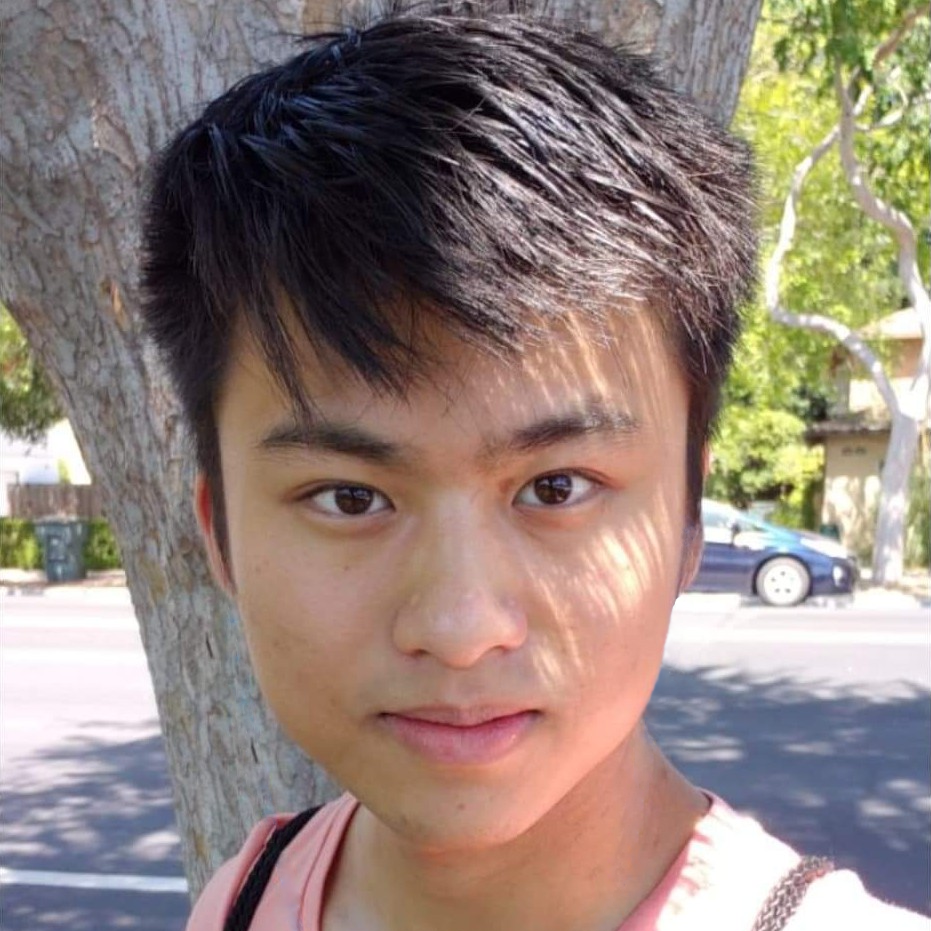
\includegraphics[height=2.3cm]{sam}
    %        \end{wrapfigure}
    %    \normalsize
    %    Sam Tenka is a grad student in computer science 
    %    at MIT.  Their email address is
    %    \texttt{
    %        c{\tiny\ }%
    %        o{\tiny\ }%
    %        l{\tiny\ }%
    %        i{\tiny@}%
    %        m{\tiny\ }%
    %        i{\tiny\ }%
    %        t{\tiny\ }%
    %        .{\tiny\ }%
    %        e{\tiny\ }%
    %        d{\tiny\ }%
    %        u%
    %    }.


\end{document}


